\subsection{Probabilité et graphe}
\hspace{\parindent} Dans cette partie, on devait faire un graphe qui représente la probabilité de gagner un jeu suivant le nombre de tas de fin autorisé.
\par Pour ce faire, on a créé deux fonctions: d'abord,une qui calcule la probabilité de gagner une partie avec un nombre de tas minimal choisi, et l'autre qui calcule toutes les probabilités avec tous les nombres possibles.
\subsubsection{stat\_reussite}
C'est la fonction qui calcule la probabilité de gagner une partie via un certain nombre de simulations. Elle prend trois arguments: le nombre de simulations, le nombre de tas minimal possible(par défaut c'est 2 cartes) et le nombre de cartes de jeu(par défaut 32 cartes).
\par Tout d'abord, on commence par vérifier que le nombre de tas minimal choisi par le joueur soit compris entre 2 et 32(pour le jeu\_32) ou 52(pour le jeu\_52). Ensuite, on réalise les simulations et on stocke le résultat dans une variable("res"). 
\par C'est maintenant qu'on doit calculer la probabilité proprement dite: pour chercher la probabilité, \emph{"on a compté le nombre de fois que notre condition est vérifiée(c'est-à-dire soit égale soit inférieure au nombre de tas minimal choisi), et on a divisé ce nombre par le nombre total de tas existants"}; en effet c'est justement la condition nécessaire pour dire qu'une partie est gagnée.
	\\
	\begin{itemize}
	\color{blue}\item[•]Aperçu du code:
	\end{itemize}
	
	\lstset{language=Python}
	\lstset{frame=lines}
	\lstset{label={lst:code_direct}}
	\lstset{basicstyle=\footnotesize}
	\begin{lstlisting}
def stat_reussite(nb_sim, nb_min_reussite=2, nb_cartes=32):
    prob = None
    if (nb_min_reussite >= 2 and nb_min_reussite <= nb_cartes):
        res = res_multi_simulation(nb_sim, nb_cartes)
        count = 0
        for i in res:
            if (i <= nb_min_reussite):
                count += 1
        prob = round(count / nb_sim, 4)
        
    return prob
	\end{lstlisting}

\subsubsection{stat\_tout\_nombre}
Cette fonction est le pilier de la création du graphe de probabilité car elle calcule toutes les probabilité de victoire selon le nombre de tas minimal. Ici, on commence par calculer la probabilité de gagner en choisi un nombre minimal de 2 cartes(fin parfaite) et on augmente ce nombre au fur-et-à-mesure jusqu'à atteindre le nombre maximal autorisé, c'est-à-dire(le nombre total de cartes jouées).
\par Ainsi, on a pu stocké les résultats dans une liste pour chaque nombre de tas minimal possible. Par conséquent, on a pu obtenir un graphe ci-dessous représentant cette évolution.
	\\
	\begin{itemize}
	\color{blue}\item[•]Aperçu du code:
	\end{itemize}
	
	\lstset{language=Python}
	\lstset{frame=lines}
	\lstset{label={lst:code_direct}}
	\lstset{basicstyle=\footnotesize}
	\begin{lstlisting}
	def stat_tout_nombre(nb_sim, nb_cartes=32):
    res_stat = []
    i = 2
    while (i<=nb_cartes):
        res_stat.append(stat_reussite(nb_sim, i, nb_cartes))
        i += 1

    return res_stat
	\end{lstlisting}
	
\par Voici donc le graphe obtenu après tois différents nombres de simulations que l'on a faites:
\begin{figure}[h]
\centerline{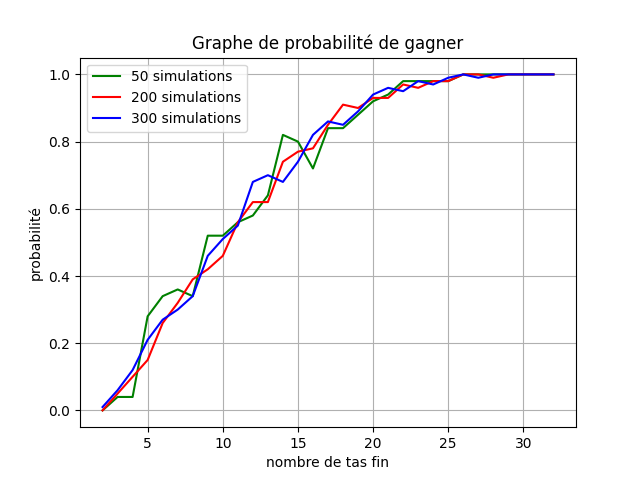
\includegraphics{graphe.png}}
\end{figure}

\par Nous remarquons ici que plus on autorise un plus grand nombre des tas final, plus la probabilité de gagner est grande. On constate aussi que la fin parfaite(2 tas) est vraiment difficile d'accès, puisque les graphes nous montre que sa probabilité est quasiment nulle.
\par En utilisant le module \emph{matplotlib}, voici comment on a pu réaliser le graphe dans la fonction principale:
	\\
	\begin{itemize}
	\color{blue}\item[•]Aperçu du code:
	\end{itemize}
	
	\lstset{language=Python}
	\lstset{frame=lines}
	\lstset{label={lst:code_direct}}
	\lstset{basicstyle=\footnotesize}
	\begin{lstlisting}
if __name__ == "__main__":

    x = linspace(2, 32, 31) #de 2 a 32, il y a 31 valeurs
    
    plt.figure()

    proba = stat_tout_nombre(50)
    proba1 = stat_tout_nombre(200)
    proba3 = stat_tout_nombre(300)

    y = []
    z = []
    w = []

    for a in proba:
        y.append(a)
    plt.plot(x,y, 'green')

    for a in proba1:
        z.append(a)
    plt.plot(x,z, 'red')

    for a in proba3:
        w.append(a)
    plt.plot(x,w, 'blue')

    plt.title("Graphe de probabilite de gagner")
    plt.xlabel("nombre de tas fin")
    plt.ylabel("probabilite")
    plt.legend(['50 simulations','200 simulations','300 simulations'])

    plt.grid()
    plt.show()
	\end{lstlisting}
\par Par ailleurs, l'on peut augmenter ces probabilités. C'est ce que l'on verra dans la partie suivante où l'on va tricher un peu dans ce jeu.